\section{Tổng quan}

Hệ thống được thiết kế theo kiến trúc \textbf{Stateful Real-time PWA}, tối ưu hóa cho trải nghiệm di động và khả năng chơi offline. Kiến trúc này không chia cắt cứng nhắc giữa các tầng mà kết nối chặt chẽ thông qua một lõi logic dùng chung (Shared Logic), đảm bảo tính đồng nhất giữa trải nghiệm người dùng và quy tắc nghiệp vụ của máy chủ.

\subsection{Sơ đồ cấu trúc hệ thống}

\begin{figure}[h!]
    \centering
    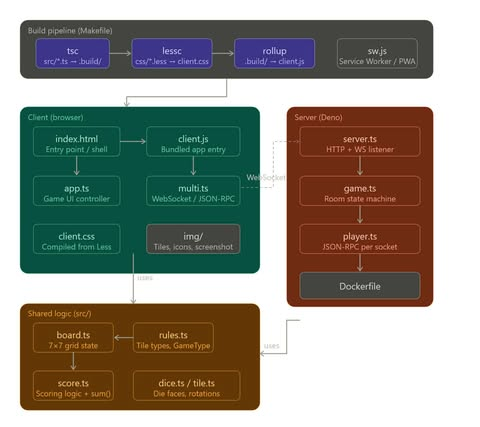
\includegraphics[width=0.8\textwidth]{images/part5/template.png}
    \caption{Kiến trúc tổng quát}
\end{figure}

Tổ chức hệ thống được phân tách thành 3 phân vùng (Panels) chức năng chính, xoay quanh một lõi domain tập trung:

\begin{itemize}[topsep=0pt, itemsep=2.5pt, leftmargin=1.5cm]
    \item Build Pipeline (Hạ tầng sản xuất - Makefile): Chuyển đổi mã nguồn (\texttt{.ts}, \texttt{.less}) thành các tài nguyên phân phối (\texttt{.js}, \texttt{.css}).
    \item Server Side (Hệ thống máy chủ - Node.js + tsx): Quản lý quyền lực (Authority), trạng thái phòng chơi (Room State), và kết nối đa người chơi qua Socket.IO.
    \item Client Side (Giao diện người dùng - Browser): Render giao diện đồ họa, xử lý tương tác trực tiếp và phản hồi tức thời (Optimistic UI).
    \item Shared Logic (Nhân Domain - \texttt{src/}): Chứa bộ luật chơi (\texttt{rules.ts}, \texttt{score.ts}). Đây là thành phần duy nhất chạy song song ở cả Client và Server để đảm bảo tính nhất quán.
\end{itemize}

\subsection{Ranh giới giữa Client và Server}

Ranh giới giữa Frontend và Backend hoạt động theo cơ chế State Synchronization (Đồng bộ trạng thái) thay vì các Request/Response tĩnh thông thường.

\subsubsection{Giao thức kết nối}

\begin{itemize}[topsep=0pt, itemsep=2.5pt, leftmargin=1.5cm]
    \item Kênh truyền dẫn: Socket.IO (WebSocket với fallback).
    \item Định dạng thông điệp: Socket.IO events. Máy chủ định nghĩa kiểu sự kiện \texttt{ClientToServerEvents} và \texttt{ServerToClientEvents} trong file \texttt{types.ts}, đảm bảo an toàn kiểu dữ liệu giữa client và server. Các module xử lý bao gồm: \texttt{rooms.ts} (lifecycle phòng), \texttt{draftEngine.ts} (draft), \texttt{timerEngine.ts} (simulation).
\end{itemize}

\subsubsection*{Các sự kiện Socket.IO chính}

\begin{longtable}{|l|l|p{10cm}|}
\hline
\rowcolor[rgb]{0.8, 0.9, 1.0}
\textbf{Loại} & \textbf{Tên sự kiện} & \textbf{Mô tả} \\
\hline
C→S & \texttt{room:create} & Tạo phòng mới và vào game ngay, có thể chọn thành phố/tutorial \\
C→S & \texttt{room:join} & Tham gia phòng theo roomId \\
C→S & \texttt{room:reconnect} & Kết nối lại phòng khi mất mạng \\
C→S & \texttt{room:leave} & Rời phòng chơi \\
C→S & \texttt{room:setReady} & Đánh dấu sẵn sàng \\
C→S & \texttt{game:start} & Bắt đầu game (sau khi tất cả sẵn sàng) \\
C→S & \texttt{matchmaking:find} & Vào hàng đợi tìm trận tự động \\
C→S & \texttt{matchmaking:cancel} & Hủy tìm trận \\
C→S & \texttt{draft:selectCard} & Chọn thẻ trong pool draft \\
C→S & \texttt{draft:confirmPick} & Xác nhận giữ thẻ và chuyển phần còn lại \\
C→S & \texttt{planning:placeCard} & Đặt thẻ vào ô (rowIndex, colIndex) \\
C→S & \texttt{planning:discardCard} & Hủy thẻ để thu hồi tài nguyên \\
C→S & \texttt{planning:payDebt} & Trả Token Nợ bằng tài nguyên \\
C→S & \texttt{planning:returnBoardCard} & Gỡ thẻ khỏi board về lại hand \\
C→S & \texttt{planning:confirm} & Chốt lịch trình ngày hiện tại \\
C→S & \texttt{tutorial:pauseReplay} & Tạm dừng replay trong tutorial \\
C→S & \texttt{tutorial:resumeReplay} & Tiếp tục replay trong tutorial \\
\hline
S→C & \texttt{room:joined} & Đã vào phòng (kèm roomId, playerId, state) \\
S→C & \texttt{room:state} & Snapshot trạng thái phòng theo từng người chơi \\
S→C & \texttt{room:left} & Đã rời phòng \\
S→C & \texttt{matchmaking:status} & Số người đang chờ trong hàng đợi (count, target) \\
S→C & \texttt{game:error} & Thông báo lỗi (hành động không hợp lệ) \\
\hline
\end{longtable}

\newpage

\subsubsection{Phân chia trách nhiệm}

Hệ thống vận hành theo nguyên lý "Optimistic Client — Authoritative Server":

\begin{table}[H]
    \centering
    \renewcommand{\arraystretch}{1.3}
    \setlength{\tabcolsep}{6pt}
    \begin{tabular}{|>{\RaggedRight\arraybackslash}p{3cm}|>{\RaggedRight\arraybackslash}p{6cm}|>{\RaggedRight\arraybackslash}p{6cm}|}
        \hline
        \rowcolor[rgb]{0.8, 0.9, 1.0}
        \textbf{Đặc điểm} & \textbf{Phía Client (Frontend)} & \textbf{Phía Server (Backend)} \\ \hline
        Vai trò chính & Trải nghiệm \& Tương tác (UX) & Quyền quyết định \& Sự thật (Authority) \\ \hline
        Xử lý Logic & Dự đoán kết quả (Preview) dựa trên Shared Logic để phản hồi UI tức thì. & Tái kiểm tra (Validate) mọi hành động gửi lên để ngăn chặn gian lận. \\ \hline
        Trạng thái & Chỉ lưu giữ trạng thái cục bộ của 1 người dùng. & Quản lý trạng thái tổng thể của cả phòng chơi (Room FSM). \\ \hline
        Lưu trữ & Caching tài nguyên qua Service Worker. & Lưu trữ trạng thái trận đấu trong bộ nhớ Node.js (In-memory). \\ \hline
    \end{tabular}
    \caption{Phân chia trách nhiệm giữa Client và Server}
\end{table}
\FloatBarrier

\subsection{Luồng tương tác giữa các vùng}

Để minh họa ranh giới này, xét quy trình khi một người chơi thực hiện nước đi:

\begin{itemize}[topsep=0pt, itemsep=2.5pt, leftmargin=1.5cm]
    \item Tại Client: \texttt{app.ts} gọi \texttt{rules.ts} (Shared) để kiểm tra hợp lệ ngay lập tức và hiển thị điểm dự kiến (0ms delay).
    \item Qua Boundary: \texttt{socketClient.ts} gửi gói tin Socket.IO event (\texttt{socket.emit}) qua WebSocket.
    \item Tại Server: \texttt{rooms.ts} tiếp nhận, \texttt{gameEngine.ts} gọi chính \texttt{rules.ts}, \texttt{board.ts}, \texttt{score.ts} (Shared) để xác thực lần cuối.
    \item Đồng bộ: Nếu hợp lệ, Server cập nhật trạng thái chung và broadcast snapshot mới nhất cho tất cả người chơi để đồng bộ hóa giao diện.
\end{itemize}

Kiến trúc này giúp dự án đạt được sự cân bằng giữa tốc độ phản hồi của ứng dụng Offline và tính bảo mật, đồng bộ của ứng dụng Online.